\section{Цель работы}
Знакомство с типовыми нелинейными звеньями.
\section{Задание на лабораторную работу}
Выполнить следующие действия выполнить над пробными сигналами (синусоида, меандр, пила) и всеми 
нелинейностями (реле, мертвая зона, насыщение)
\begin{enumerate}
	\item Сгенерировать пробный сигнал длительностью 100 секунд, построить его спектр
	\item Получить отклик типовых нелинейных звеньев на пробные сигналы, построить их спектры
	\item Построить статическую характеристику нелинейного звена, объяснить разницу при разных пробных сигналах
	\item Получить отклик линейного звена на преобразованный сигнал, построить его спектр
	\item Изменить последовательность НЭ-ЛЗ на ЛЗ-НЭ, получить результирующий сигнал, построить его спектр
\end{enumerate}
\section{Основные теоретические положения}
\subsection{Пробные сигналы}
\subsubsection{Синусоида}
Синусоидальное изменение какой-либо величины (рис. \ref{fig:1}) называется гармоническим колебанием 
Примерами могут являться любые колебательные процессы начиная от качания маятника и кончая звуковыми волнами 
(гармонические колебания воздуха) — колебания напряжения в электрической сети переменного тока, 
изменение тока и напряжения в колебательном контуре и др
\begin{figure}[H]
	\centering
	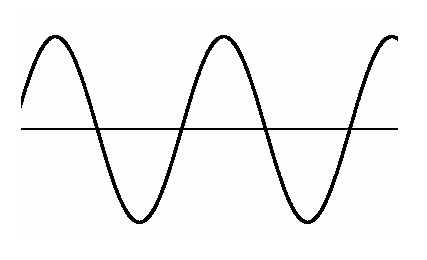
\includegraphics[width=0.5\linewidth]{body/templates/sine.png}
	\caption{Синусоида}
	\label{fig:1}
\end{figure}

Для вопросов теории автоматического управления синусоида имеет интерес вследствие того, 
что является базисной функцией преобразования Фурье. И, соответственно, 
спектр такого сигнала имеет значение только в одном отсчете частотной характеристики, 
что делает его идеальным для получения частотной характеристики объекта.

Для формирования синусоиды в Python используется функция sin(t) библиотеки NumPy:

\texttt{sig\textunderscore sin = np.sin(t)}
\subsubsection{Меандр}
Меандр (по названию геометрического орнамента в виде ломаной линии) — периодический сигнал
прямоугольной формы (рис. \ref{fig:2}), широко используемый в радиотехнике. Длительность импульса
и длительность паузы в периоде такого сигнала равны. Другими словами, меандр — периодический
прямоугольный сигнал с коэффициентом заполнения, равным 0,5
\begin{figure}[H]
	\centering
	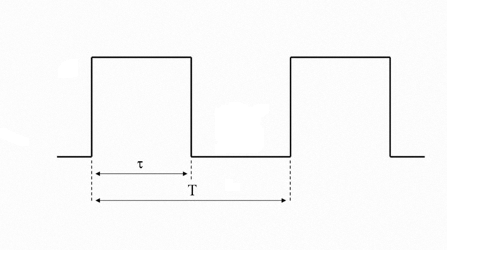
\includegraphics[width=0.5\linewidth]{body/templates/meandr.png}
	\caption{Меандр}
	\label{fig:2}
\end{figure}

Спектр меандра пропорционален функции sinc(x). Меандр может быть двухполярным (спектр описывается
функцией sinc(x)) и однополярным (sinc(x) + 1)

Сигнал приближённо такого вида (с ненулевой длительностью фронтов и спадов) создаётся различными
мультивибраторами (на транзисторах, логических элементах, операционных усилителях)

Для формирования меандра в Python используется функция square(t) из библиотеки signal пакета SciPy:

\texttt{sig\textunderscore meandr = signal.square(t)}
\subsubsection{Пила}
Пилообразный сигнал является последовательностью пилообразных импульсов. Имеет более растянутую
спектральную характеристику, чем меандр, что позволяет сигналом одной частоты анализировать
отклик объекта на большем числе частот
\begin{figure}[H]
	\centering
	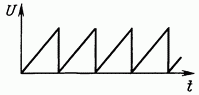
\includegraphics[width=0.5\linewidth]{body/templates/sawtooth.png}
	\caption{Пила}
	\label{fig:3}
\end{figure}

Для формирования пилообразного сигнала в Python используется функция sawtooth(t) из библиотеки signal пакета SciPy:

\texttt{sig\textunderscore saw = signal.sawtooth(t)}
\subsection{Типовые нелинейные звенья}
\subsubsection{Идеальное реле (знак)}
Нелинейность \textquotedblleftИдеальное реле\textquotedblright\ позволяет учесть в моделях одноименных электромеханические механизмы
или их электронные аналоги (транзисторы и др.), кроме того такая нелинейность необходима
для описания физических процессов не зависящих от амплитуды, но зависящих от знака
воздействия (например, сухое трение). Статическая характеристика представлена на рис. \ref{fig:4}
\begin{figure}[H]
	\centering
	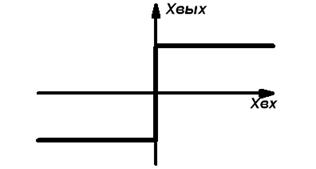
\includegraphics[width=0.5\linewidth]{body/templates/relay.png}
	\caption{Статическая характеристика нелинейности \textquotedblleftИдеальное реле\textquotedblright}
	\label{fig:4}
\end{figure}

Для формирования Нелинейность \textquotedblleftИдеальное реле\textquotedblright\ в Python используется функция sign(x(t)) из библиотеки NumPy:

\texttt{sig\textunderscore XXX\textunderscore after\textunderscore relay = np.sign(sig\textunderscore XXX)}
\subsubsection{Мертвая зона}
Мертвой зоной принято называть неединственность положения равновесия
(y = const, u = const => dy/dt = 0, du/dt = 0). Примером объекта с такой нелинейностью может
служить маятник. Нелинейность подобного рода приводит к конечности временных процессов.
Статическая характеристика представлена на рис. \ref{fig:5}.
\begin{figure}[H]
	\centering
	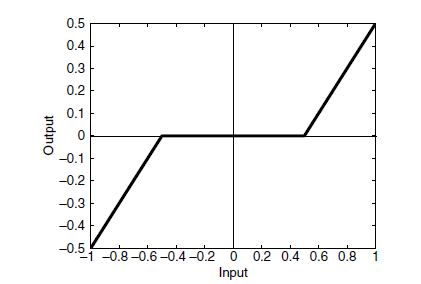
\includegraphics[width=0.5\linewidth]{body/templates/dead-zone.png}
	\caption{Статическая характеристика нелинейности \textquotedblleftМертвая зона\textquotedblright}
	\label{fig:5}
\end{figure}

Нелинейность \textquotedblleftМертвая зона\textquotedblright\ позволяет учесть малые значения отклонений.

Для реализации нелинейности \textquotedblleftМертвая зона\textquotedblright\ в Python также необходимо реализовать функцию самостоятельно,
а также векторизовать ее с помощью функции np.vectorize:

\texttt{def dead\textunderscore zone\textunderscore scalar(x, width = 0.5):}

\texttt{\hspace{10mm}if np.abs(x)<width:}

\texttt{\hspace{20mm}return 0}

\texttt{\hspace{10mm}elif x>0:}

\texttt{\hspace{20mm}return x-width}

\texttt{\hspace{10mm}else:}

\texttt{\hspace{20mm}return x+width}

\texttt{dead\textunderscore zone = np.vectorize(dead\textunderscore zone\textunderscore scalar,}

\texttt{otypes=[np.float])}

Векторизация — это прием ускорения вычислений, заключающийся в переходе от циклов к матричным (векторным) вычислениям
После создания функции задача сводится к применению полученной функции к сигналу:

\texttt{sig\textunderscore XXX\textunderscore after\textunderscore dead\textunderscore zone = dead\textunderscore zone(sig\textunderscore XXX)}
\subsubsection{Усилитель с насыщением}
Ограниченность уровня переменных связана в первую очередь с различными физическими ограничениями, 
препятствующими бесконечному росту переменных состояния, например вязкое трение (пренебрежимо малое
при малых скоростях и имеющее квадратичный рост на больших) или различные процессы, связанные с насыщением. 
Статическая характеристика представлена на рис. \ref{fig:6}.

Принцип работы такой нелинейности заключается в пропуске сигнала только до уровня предельной амплитуды.

Нелинейность \textquotedblleftНасыщение\textquotedblright\ позволяет учесть большие значения переменных.
\begin{figure}[H]
	\centering
	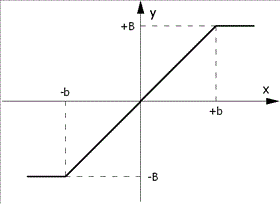
\includegraphics[width=0.5\linewidth]{body/templates/saturation.png}
	\caption{Статическая характеристика нелинейности \textquotedblleftНасыщение\textquotedblright}
	\label{fig:6}
\end{figure}

Для реализации нелинейности \textquotedblleftНасыщение\textquotedblright\ в Python также необходимо реализовать функцию самостоятельно, 
а также векторизовать ее с помощью функции np.vectorize:

\texttt{def saturation\textunderscore scalar(x, hight = 0.5):}

\texttt{\hspace{10mm}if np.abs(x)<hight:}

\texttt{\hspace{20mm}return x}

\texttt{\hspace{10mm}elif x>0:}

\texttt{\hspace{20mm}return hight}

\texttt{\hspace{10mm}else:}

\texttt{\hspace{20mm}return -hight}

\texttt{saturation = np.vectorize(saturation\textunderscore scalar, oty}

\texttt{pes=[np.float])}

Далее применяем функцию к сигналу:

\texttt{sig\textunderscore XXX\textunderscore after\textunderscore saturation = saturation(sig\textunderscore XXX)}
\subsection{Фильтрация сигнала}
Фильтр — устройство (блок) для выделения желательных компонентов спектра сигнала и/или подавления нежелательных, 
фактически может представлять из себя любое звено с подходящей АЧХ.

В этой работе для фильтрации сигналов будем использовать простейший фильтр нижних частот — 
инерционное звено первого порядка, реальным аналогом которого служит, например, RC-фильтр.

Такие фильтры являются БИХ, для их применения в SciPy имеется функция scipy.signal.lfilter:

\texttt{k = 1}

\texttt{T = 1}

\texttt{B = [ k/(1+T/0.01) ]}

\texttt{A = [1, -1/(1+0.01/T)]}

\texttt{filtered\textunderscore sig\textunderscore XXX\textunderscore after\textunderscore YYY=signal.lfilter(B,A,np.sign(si}

\texttt{g\textunderscore XXX\textunderscore after\textunderscore YYY))}
\subsection{Построение спектра сигналов}

Для построения спектра дискретных сигналов берется модуль от дискретного (быстрого) преобразования Фурье сигнала.

В Python:

\texttt{sig\textunderscore spec = np.abs(fft(sin))}

Заметим, что при формировании спектра таким образом он является репрезентативным только на отрезке [0, T/2], 
где T — частота дискретизации. Кроме того необходимо получить значения частот для отсчетов дискретного преобразования Фурье:

В Python имеется функция:

\texttt{freqs = np.fft.fftfreq(<Размер вектора сигнала>, }

\texttt{<Период дискретизации>)}

\section{Обработка результатов эксперимента}

Вариант номер 14

Амплитуда тестового сигнала: 2.4

Частота тестового сигнала: 50 Гц

Длительность тестового сигнала: 100 с

Параметр нелинейностей 1: 1.9

Коэффициент усиления линейного звена: 4.7

Постоянная времени линейного звена: 2.9

Период дискретизации сигнала: 0.00001 с

\subsection{Пробные сигналы}

На рис. \ref{fig:7} представлена чистая синусоида и её спектр. Значение амплитуды сигналы
составляет 2.4, а частоты - 50 Гц. Спектр построенного синусоидального сигнала является
спичкой на частоте 50 Гц

\begin{figure}[H]
	\centering
	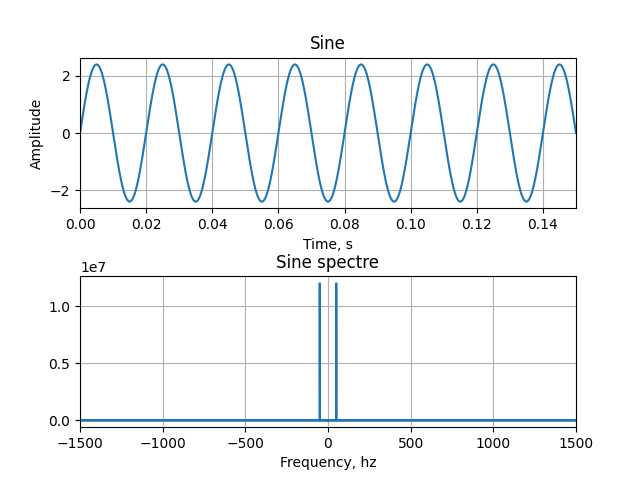
\includegraphics[width=0.7\linewidth]{body/images/sine-and-its-spectre.png}
	\caption{Синусоида и её спектр}
	\label{fig:7}
\end{figure}

На рис. \ref{fig:8} представлен меандр скважностью 0.5 и его спектр.
Появление дополнительных гормоник на спектре обусловлено наличием нечетных гармоник в его
разложении в ряд Фурье, с амплитудой, уменьшающейся пропорционально их номеру

\begin{figure}[H]
	\centering
	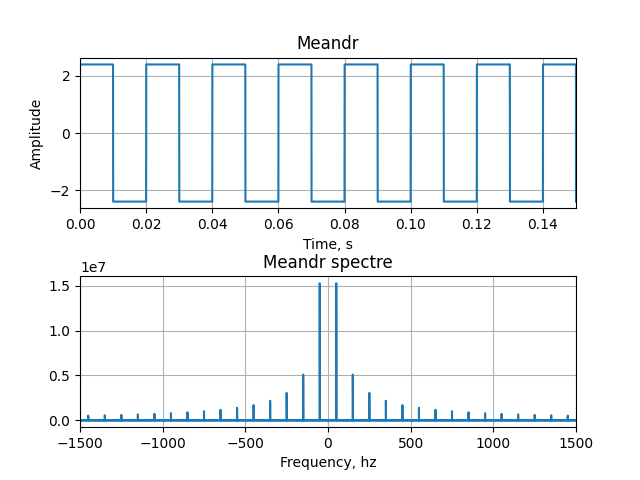
\includegraphics[width=0.7\linewidth]{body/images/meandr-and-its-spectre.png}
	\caption{Меандр и его спектр}
	\label{fig:8}
\end{figure}

На рис. \ref{fig:9} представлен пилообразный сигнал и его спектр.
Спектр соответствует спектру меандра, но со включенными, помимо нечетных, четными гармониками

\begin{figure}[H]
	\centering
	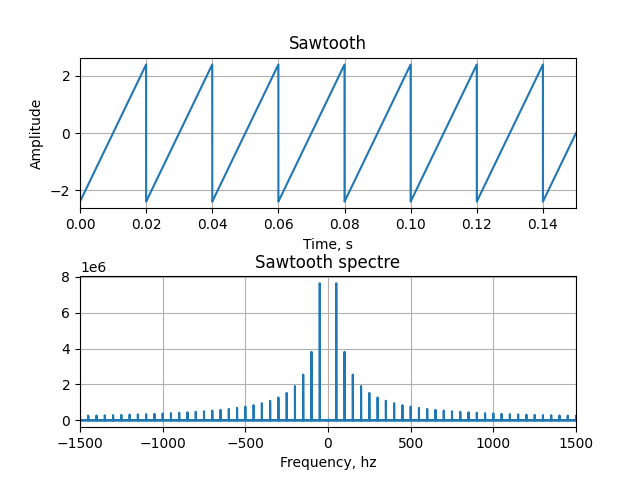
\includegraphics[width=0.7\linewidth]{body/images/sawtooth-and-its-spectre.png}
	\caption{Пила и ее спектр}
	\label{fig:9}
\end{figure}

\subsection{Статические характеристики нелинейностей}


\subsubsection{Статические характеристики \textquotedblleftИдеального реле\textquotedblright}

\begin{figure}[H]
	\centering
	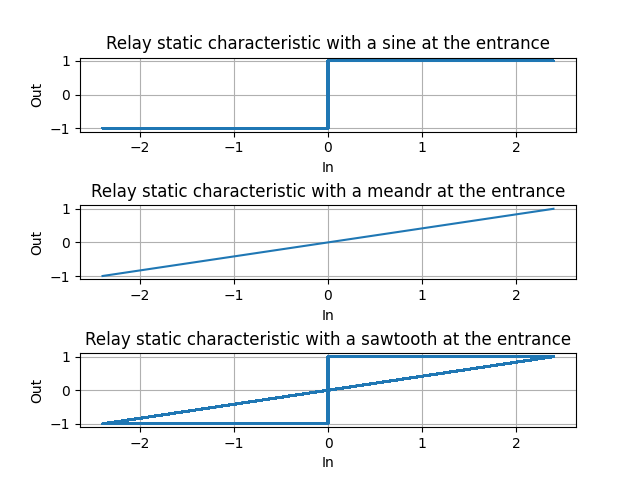
\includegraphics[width=0.7\linewidth]{body/images/relay-static-characteristics.png}
	\caption{Статические характеристики нелинейности \textquotedblleftИдеальное реле\textquotedblright}
	\label{fig:10}
\end{figure}

На рис. \ref{fig:10} представлена статическая характеристика
нелинейности \textquotedblleftИдеальное реле\textquotedblright\ 
при подаче разных сигналов: синусиоды, мендра и пилы.
Статическая характеристика показывает, что, при отрицательных
входах, выход будет равен -1, а при положительных входах выход
будет равен 1. Синусоида сформировала ту же характеристику, что
и линейный возрастающий сигнал, используемый в теоретическом
описании нелинейности \textquotedblleftИдеального реле\textquotedblright, представляющую собой
монотонную прямую с рызрывом первого рода в точке 0. При подаче
меандра статическая характеристика приобрела вид наклонной прямой,
соединяющий две точки, соответствующие двум значениям, в которых
мог бы находится график мендра. Пилообразный сигнал же скомбинировал
в себе черты первой и второй характеристик, так как наличие
наклонного переднего фронта аналогично наличию линейно
возрастающего сигнала, а вертикальный задний фронт соответствует
скачку между значениями, что характерно для меандра

\subsubsection{Статические характеристики нелинейности \textquotedblleftМёртвая зона\textquotedblright}

\begin{figure}[H]
	\centering
	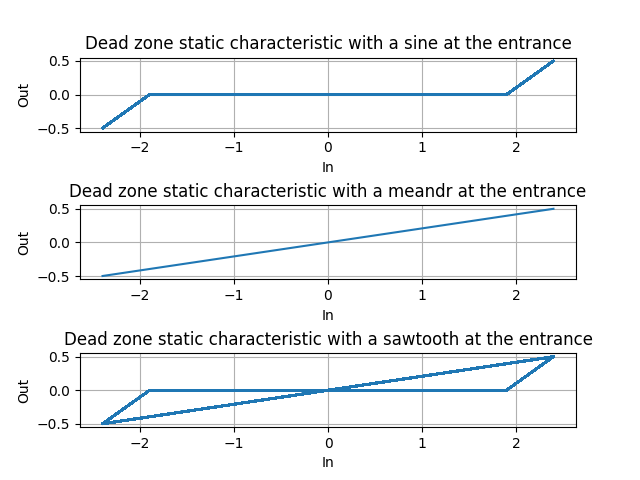
\includegraphics[width=0.7\linewidth]{body/images/dead-zone-static-characteristics.png}
	\caption{Статические характеристики нелинейности \textquotedblleftМёртвая зона\textquotedblright}
	\label{fig:11}
\end{figure}

На рис. \ref{fig:11} представлена статическая характеристика
нелинейности \textquotedblleftМёртвая зона\textquotedblright\ при подаче разных сигналов: синусиоды, мендра
и пилы. По этой статической характеристике видно, что все статические
характеристики получили отличными друг от друга. Синусоида
сформировала ту же характеристику, что и линейный возрастающий
сигнал, используемый в теоретическом описании нелинейности
\textquotedblleftМёртвая зона\textquotedblright, представляющую из себя линейно возрастающую
функцию, которая смещается на 3.8 на значении 0. При подаче меандра
статическая характеристика приобрела вид наклонной прямой,
соединяющий две точки, соответствующие двум значениям, в которых
мог бы находится график мендра. Пилообразный сигнал же скомбинировал
в себе черты первой и второй характеристик, так как наличие
наклонного переднего фронта аналогично наличию линейно
возрастающего сигнала, а вертикальный задний фронт соответствует
скачку между значениями, что характерно для меандра

\subsubsection{Статические характеристики нелинейности \textquotedblleftНасыщение\textquotedblright}

\begin{figure}[H]
	\centering
	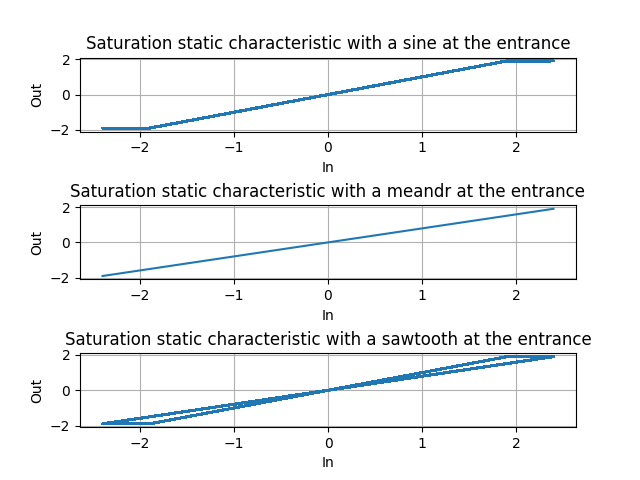
\includegraphics[width=0.7\linewidth]{body/images/saturation-static-characteristics.png}
	\caption{Статические характеристики нелинейности \textquotedblleftНасыщение\textquotedblright}
	\label{fig:12}
\end{figure}

На рис. \ref{fig:12} представлена статическая характеристика
нелинейности \textquotedblleftНасыщение\textquotedblright\ при подаче разных сигналов: синусиоды, мендра
и пилы. По этой статической характеристике видно, что все статические
характеристики получили отличными друг от друга. Синусоида
сформировала ту же характеристику, что и линейный возрастающий
сигнал, используемый в теоретическом описании нелинейности
\textquotedblleftНасыщение\textquotedblright, представляющую из себя линейно возрастающую
функцию, которая рассекается на значениях -1.9 и 1.9.
При подаче меандра статическая характеристика приобрела вид
наклонной прямой, соединяющий две точки, соответствующие двум
значениям, в которых мог бы находится график мендра.
Пилообразный сигнал же скомбинировал в себе черты первой
и второй характеристик, так как наличие наклонного переднего
фронта аналогично наличию линейно возрастающего сигнала,
а вертикальный задний фронт соответствует скачку между
значениями, что характерно для меандра

\subsection{Получение откликов типовых нелинейных звеньев на пробные сигналы.
Получение спектров откликов}

\subsubsection{Нелинейность \textquotedblleftИдеальное реле\textquotedblright}

После прохождения нелинейности \textquotedblleftИдеальное реле\textquotedblright\
сигнал приобретает форму меандра, амплитуда которого по модулю равна 1. Сам же
сигнал остаётся на той же частоте

\begin{figure}[H]
	\centering
	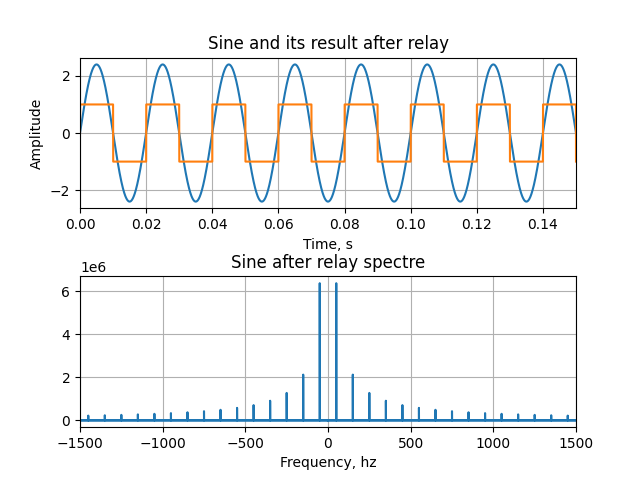
\includegraphics[width=0.75\linewidth]{body/images/sine-after-relay-and-its-spectre.png}
	\caption{График синусоиды и отклик нелинейности 
	\textquotedblleftИдеальное реле\textquotedblright\ на неё. Спектр отклика}
	\label{fig:13}
\end{figure}

На рис. \ref{fig:13} представлена синусоида до и после прохождения
нелинейности \textquotedblleftИдеальное реле\textquotedblright, 
а также спектр преобразованного сигнала. Синусоида после прохождения
нелинейности \textquotedblleftИдеальное реле\textquotedblright\
преобразилась до вида меандра, имеющего ту же частоту, что и пробный
сигнал. Это отражается на спектре: в нём становится больше гармоник,
— это обуславливается дополнительными преобразованиями меандра до
синусоиды. Амплитуда же полученного меандра не соответствует
амплитуде поданной синусоиды - это отличительная особенность 
нелинейности \textquotedblleftИдеальное реле\textquotedblright.
Амплитуда выходного сигнала по модулю будет равна 1. Это заметно
и на спектре, где главная гармоника уменьшилась в своей мощности 

\begin{figure}[H]
	\centering
	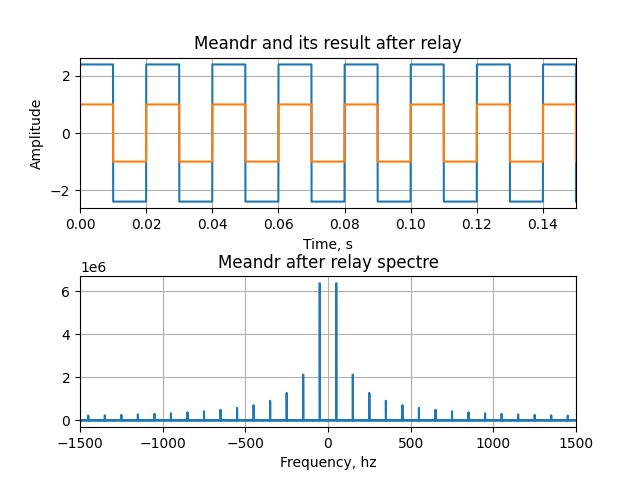
\includegraphics[width=0.75\linewidth]{body/images/meandr-after-relay-and-its-spectre.png}
	\caption{График меандра и отклик нелинейности 
	\textquotedblleftИдеальное реле\textquotedblright\ на него. Спектр отклика}
	\label{fig:14}
\end{figure}

На рис. \ref{fig:14} представлен меандр до и после прохождения
нелинейности \textquotedblleftИдеальное реле\textquotedblright,
а также спектр преобразованногосигнала. Меандр после прохождения
нелинейности \textquotedblleftИдеальное реле\textquotedblright\ 
лишь изменяет свою ампилитуду, что видно и на спектре: все
гармоники теряют в своей мощности

\begin{figure}[H]
	\centering
	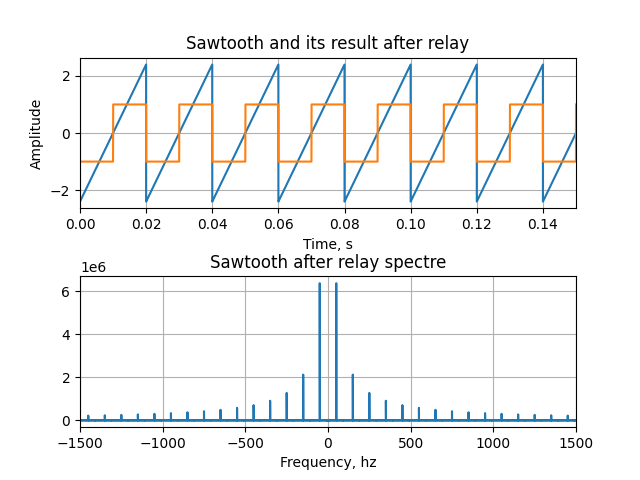
\includegraphics[width=0.75\linewidth]{body/images/sawtooth-after-relay-and-its-spectre.png}
	\caption{График пилы и отклик нелинейности 
	\textquotedblleftИдеальное реле\textquotedblright\ на неё. Спектр отклика}
	\label{fig:15}
\end{figure}

На рис. \ref{fig:15} представлена пила до и после прохождения
нелинейности \textquotedblleftИдеальное реле\textquotedblright, а
также спектр преобразованного сигнала. Пила после прохождения нелинейности 
\textquotedblleftИдеальное реле\textquotedblright\ преобразилась
до вида меандра, имеющего ту же частоту, что и пробный сигнал.
Амплитуда выходного сигнала по модулю равна 1.
Несмотря, что амплитуда получаемого на выходе меандра имеет
меньшую амплитуду, нежели исходная пила, каждая из гармоник
меандра мощнее гармоники пилы на той же частоте. Также и самих
гармоник стало в два раза больше. Это обусловлено тем, что
пила \textquotedblleftдальше\textquotedblright\ по виду от
синусоиды. Нечётные гармоники пилы - отрисовка 
\textquotedblleftвыступающих за меандр\textquotedblright\
частей пилы. Из-за наклонной части пилы, находящейся 
\textquotedblleftпод меандром\textquotedblright\
на спектре и видно, что гармоники меандра мощнее гармоник
пилы на той же частоте

\subsubsection{Нелинейность \textquotedblleftМёртвая зона\textquotedblright}

\begin{figure}[H]
	\centering
	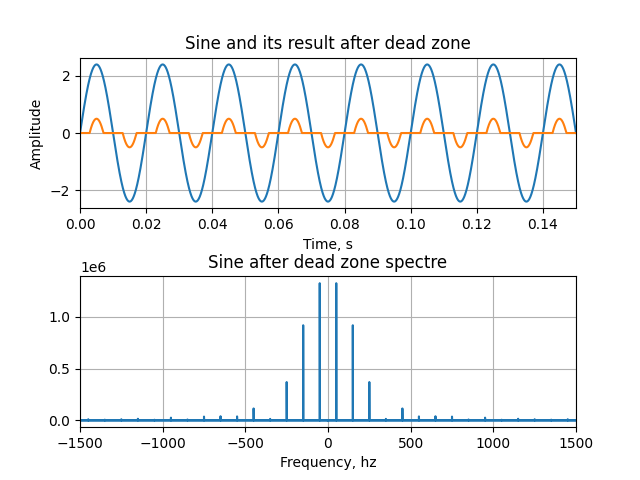
\includegraphics[width=0.75\linewidth]{body/images/sine-after-dead-zone-and-its-spectre.png}
	\caption{График синусоиды и отклик нелинейности
	\textquotedblleftМёртвая зона\textquotedblright\ на неё. Спектр отклика}
	\label{fig:16}
\end{figure}

На рис. \ref{fig:16} представлена синусоида до и после прохождения
нелинейности \textquotedblleftМёртвая зона\textquotedblright, а
также спектр преобразованного сигнала. После прохождения
нелинейности \textquotedblleftМёртвая зона\textquotedblright\ 
синусоида \textquotedblleftвжимается\textquotedblright\ в ось
абсцисс. Это отражается и на спектре: главная гармоника синусоиды
теряет в мощности и появляются дополнительные гармоники, обусловенные
неканоническим видом синусоиды после прохождения нелинейности
\textquotedblleftМёртвая зона\textquotedblright

\begin{figure}[H]
	\centering
	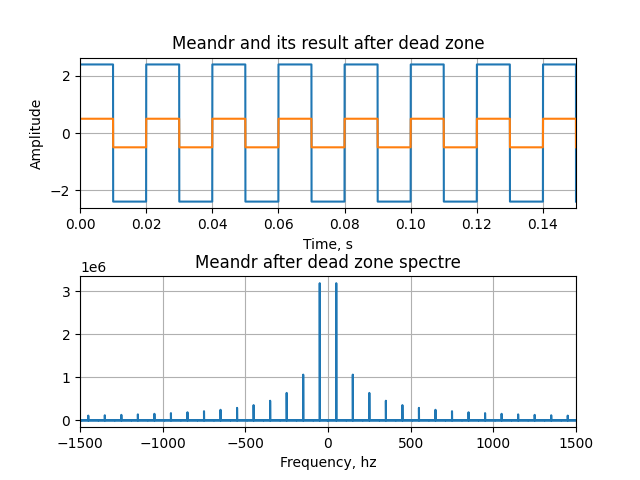
\includegraphics[width=0.75\linewidth]{body/images/meandr-after-dead-zone-and-its-spectre.png}
	\caption{График меандра и отклик нелинейности
	\textquotedblleftМёртвая зона\textquotedblright\ на него. Спектр отклика}
	\label{fig:17}
\end{figure}

На рис. \ref{fig:17} представлен меандр до и после прохождения
нелинейности \textquotedblleftМёртвая зона\textquotedblright, а
также спектр преобразованного сигнала. После прохождения
нелинейности \textquotedblleftМёртвая зона\textquotedblright\ 
меандр меняет лишь свою амплитуду, что видно и на спектре:
гармоники теряют в мощности

\begin{figure}[H]
	\centering
	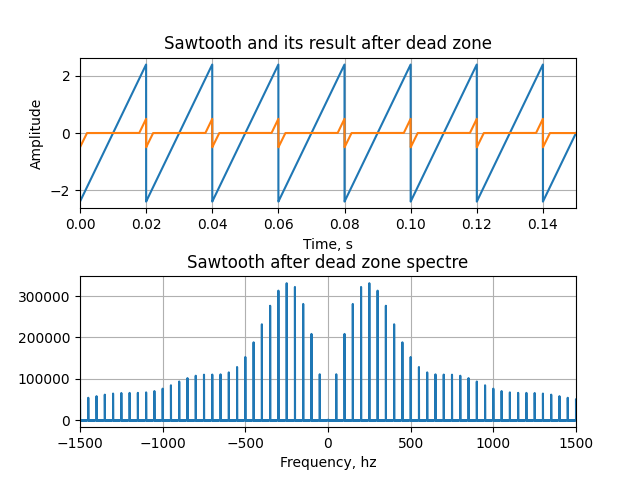
\includegraphics[width=0.75\linewidth]{body/images/sawtooth-after-dead-zone-and-its-spectre.png}
	\caption{График пилы и отклик нелинейности
	\textquotedblleftМёртвая зона\textquotedblright\ на неё. Спектр отклика}
	\label{fig:18}
\end{figure}

На рис. \ref{fig:18} представлена пила до и после прохождения
нелинейности \textquotedblleftМёртвая зона\textquotedblright, а
также спектр преобразованного сигнала. После прохождения
нелинейности \textquotedblleftМёртвая зона\textquotedblright\ 
пила \textquotedblleftвжимается\textquotedblright\ в ось
абсцисс. Это отражается и на спектре: все гармоники теряют
в мощности; основная и ближайшие к ней гармоники подавляются
сильнее остальных, в результате чего частота новой основной
гармоники стала выше частоты изначальной основной гармоники

\subsubsection{Нелинейность \textquotedblleftНасыщение\textquotedblright}

\begin{figure}[H]
	\centering
	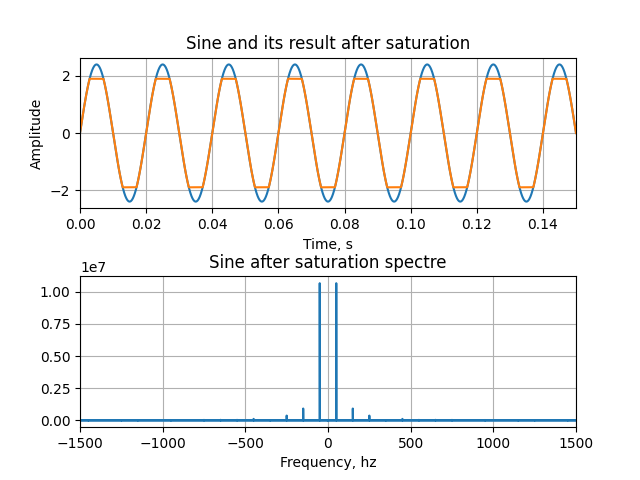
\includegraphics[width=0.75\linewidth]{body/images/sine-after-saturation-and-its-spectre.png}
	\caption{График синусоиды и отклик нелинейности
	\textquotedblleftНасыщение\textquotedblright\ на неё. Спектр отклика}
	\label{fig:19}
\end{figure}

На рис. \ref{fig:16} представлена синусоида до и после прохождения
нелинейности \textquotedblleftНасыщение\textquotedblright, а
также спектр преобразованного сигнала. После прохождения
нелинейности \textquotedblleftНасыщение\textquotedblright\ 
синусоида потеряла небольшую часть амплитуды. Верхняя часть
каждого \textquotedblleftлепестка\textquotedblright\ синусоиды срезалась
под действием нелинейности \textquotedblleftНасыщение\textquotedblright.
На спектре же данное преобразование отражается потерей
главной гармоникой небольшой части своей мощности, а также
добавлением нескольких более высокочастотных гармоник. Это
обусловлено тем, что срезанная нелинейностью
\textquotedblleftНасыщение\textquotedblright\ часть должна быть
восстановлена для получения канонического вида сигнала
синосоидальной формы. Так как эта срезанная часть мала
в моей работе, то и, соответственно, гармоники имеют невысокую
мощность и численность

\begin{figure}[H]
	\centering
	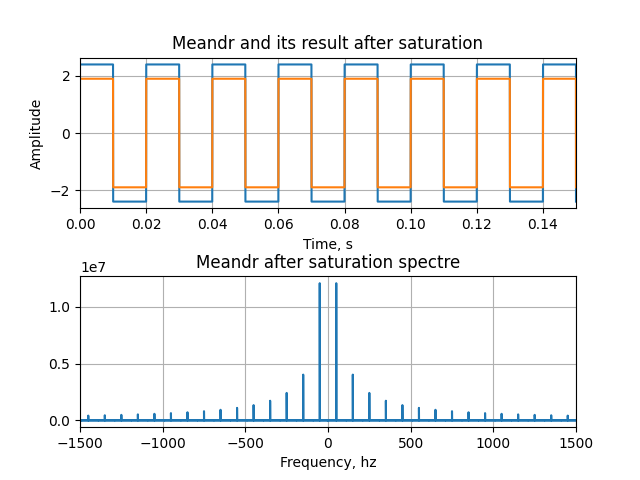
\includegraphics[width=0.75\linewidth]{body/images/meandr-after-saturation-and-its-spectre.png}
	\caption{График меандра и отклик нелинейности
	\textquotedblleftНасыщение\textquotedblright\ на него. Спектр отклика}
	\label{fig:20}
\end{figure}

На рис. \ref{fig:17} представлен меандр до и после прохождения
нелинейности \textquotedblleftНасыщение\textquotedblright, а
также спектр преобразованного сигнала. После прохождения
нелинейности \textquotedblleftНасыщение\textquotedblright\ 
меандр лишь изменяет свою ампилитуду, что видно и на спектре:
все гармоники теряют в своей мощности

\begin{figure}[H]
	\centering
	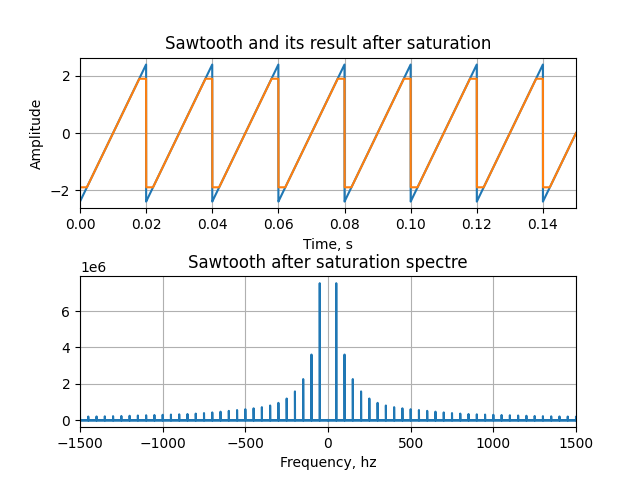
\includegraphics[width=0.75\linewidth]{body/images/sawtooth-after-saturation-and-its-spectre.png}
	\caption{График пилы и отклик нелинейности
	\textquotedblleftНасыщение\textquotedblright\ на неё. Спектр отклика}
	\label{fig:21}
\end{figure}

На рис. \ref{fig:18} представлена пила до и после прохождения
нелинейности \textquotedblleftНасыщение\textquotedblright, а
также спектр преобразованного сигнала. После прохождения
нелинейности \textquotedblleftНасыщение\textquotedblright\ 
пила потеряла небольшую часть амплитуды. Верхняя часть
каждого \textquotedblleftзубчика\textquotedblright\ пилы срезалась
под действием нелинейности \textquotedblleftНасыщение\textquotedblright.
На спектре же данное преобразование, на первый взгляд, отражается
лишь потерей амплитуды каждой из гармоник. В этой работе тяжело
различить изменения, которые связаны со срезанием части каждого
\textquotedblleftзубчика\textquotedblright\ пилы, так как сам
пилообразный сигнал обладает очень отдалённой формой синосоиды, а
поэтому и количество гармоник получается невероятно большим. В
связи с этим и входными данными варианта я не могу однозначно
утверждать о идентичности спектров, не рассматривая разницу по
амплитуде

\subsubsection{Выводы}

Из вышерассмотренных комбинаций нелинейностей и сигналов, можно
высказать несколько выводов.
При воздействии на исходный сигнал нелинейности
\textquotedblleftИдеальное реле\textquotedblright\ лучше всего
себя показывает меандр, который изменяет только лишь свою амплитуду,
а, как следствие, спектр до и после воздействия нелинейности
\textquotedblleftИдеальное реле\textquotedblright\ изменяет лишь
мощность гармоник, не меняя их частоту и не добавляя новые.
При воздействии на исходный сигнал нелинейности
\textquotedblleftМёртвая зона\textquotedblright\ было выяснено,
что исходный сигнал \textquotedblleftвдавливается\textquotedblright\ в ось
абсцисс. Меандр не очень чувствителен к таким преобразованиям 
нелинейности \textquotedblleftМёртвая зона\textquotedblright, так как
имеет мгновенное изменение сигнала, похожее на разрывы первого
рода. Из-за этого нелинейность \textquotedblleftМёртвая зона\textquotedblright\
действует только на ампилитуду меандра, не имея возможность
\textquotedblleftвдавливить\textquotedblright\ его в ось
абсцисс из-за отсутствия наклона сигнала. На спектрах синусоиды и
пилы нелинейность \textquotedblleftМёртвая зона\textquotedblright\ отражается
особенно ярко: в спектр синусоиды добавляются гармоники, а главная гармоника
теряет в амплитуде; в спектре же пилы происходят ещё большие изменения.
Эти изменения выглядят так: главная и ближайшие к ней гармоники
подавляются, а главной гармоникой становится более высокочастотная
гармоник; все гармоники теряют в мощности
При воздействии на исходный сигнал нелинейности
\textquotedblleftНасыщение\textquotedblright\ было выяснено, что
синусоида робастна к воздействию этой нелинейности. Синусоида
после прохождения нелинейности \textquotedblleftНасыщение\textquotedblright\
лишь немного теряет в амплитуде и приобретает несоклько высокочастотных
и маломощных гармоник, которые компенсируют срезанную нелинейностью
часть. Меанд по прежнему проявляет себя лучше всех. Как и в случае
с вышерассмотренными нелинейностями, меандр теряет в амплитуде, что
отражает и на спектре - все гармоники теряют в мощности. Тем не
менее никаких дополнительных гармоник не возникает, что говорит
о устойчивости этого сигнала к нелинейностям. Пилообразный сигнал
при отображённой вычислительной мощности, рассчитанной на 
100 000 точек, не изменяется даже при детальнейшем рассмотрении.
Возможно при большем количестве точек и большем срезе
каждого из \textquotedblleftзубчиков\textquotedblright\ пилы
можно было бы получить более наглядные результаты
Как итог, можно сказать, что меандр проявил себя лучше всех при
взаимодействии с такими нелинейностями, как
\textquotedblleftИдеальное реле\textquotedblright,
\textquotedblleftМёртвая зона\textquotedblright,
\textquotedblleftНасыщение\textquotedblright. После их
воздействия он теряет своей амплитуды, а на спектре изменения
касаются только мощности гармоник

\subsection{Получение откликов линейного звена на преобразованный
нелинейным звеном сигнал. Получение спектров откликов}

\subsubsection{Получение откликов линейного звена на преобрзаованный
нелинейностью \textquotedblleftИдеальное реле\textquotedblright\ сигнал.
Получение спектров откликов}

\begin{figure}[H]
	\centering
	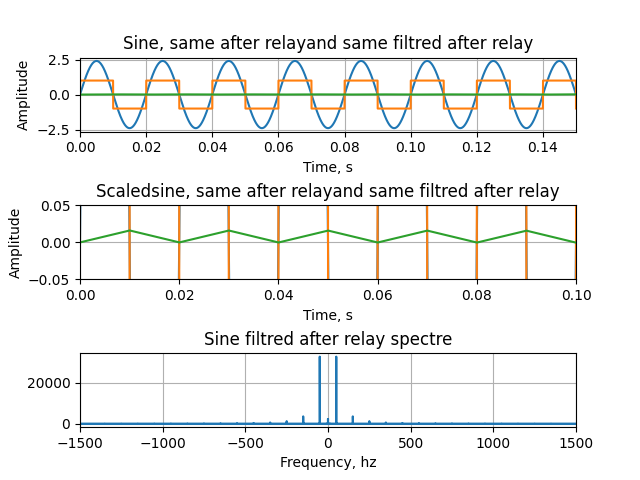
\includegraphics[width=0.95\linewidth]{body/images/sine-after-filtred-relay-and-its-spectre.png}
	\caption{График синусоиды, отклика нелинейности и отклика линейного звена на преобразованный
	нелинейностью сигнал. Спектр отклика линейного звена}
	\label{fig:22}
\end{figure}

На рис. \ref{fig:22} представлена синусоида, она же после прохождения
нелинейности \textquotedblleftИдеальное реле\textquotedblright\ и синусоида,
пропущенная последовательно через нелинейность \textquotedblleftИдеальное реле\textquotedblright\
и линейное фильтрующее звено, а также спектр преобразованного сигнала.
После прохождения нелинейности \textquotedblleftИдеальное реле\textquotedblright, а
затем фильтрующего звена, преобразований сигнал становится значительно подавлен,
но не становится монотонной прямой - это видно на детальном рассмотрении сигнала.
Результирующий сигнал напоминает своей формой асимтотически построенную синусоиду,
сдвинутую по фазе на половину периода исходной синусоиды. Касательно амплитуды,
полученный сигнал значительно потерял в амлитуде. На спектре же его главной
гармоникой по-прежнему остаётся гармоника частоты первоначальной синусоиды,
но мощность этой гармоники значительно уменьшилась. Также и самих гармоник
после фильтрации относительно преобразованной нелинейностью
\textquotedblleftИдеальное реле\textquotedblright\ синусоиды становится
меньше. Это обусловлено большей схожестью полученного сигнала с каноническим
видом синусоиды, которая смещена на значение равное своей амплитуде.
Заметна и появившаяся невероятно низкочастотная гармоника

\begin{figure}[H]
	\centering
	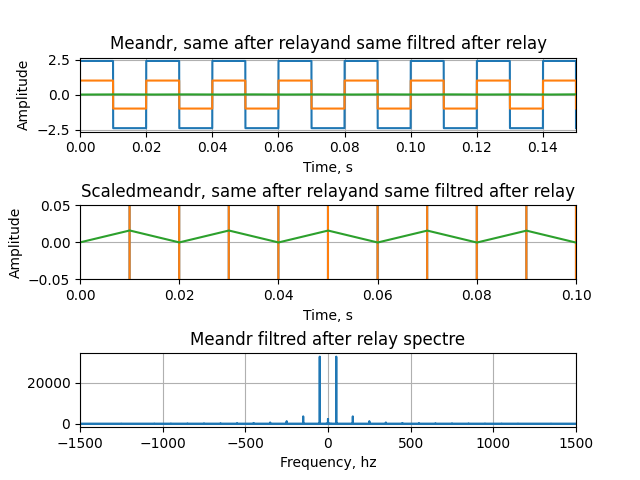
\includegraphics[width=0.95\linewidth]{body/images/meandr-after-filtred-relay-and-its-spectre.png}
	\caption{График меандра, отклика нелинейности и отклика линейного звена на преобразованный
	нелинейностью сигнал. Спектр отклика линейного звена}
	\label{fig:23}
\end{figure}

На рис. \ref{fig:23} представлен меандр, он же после прохождения
нелинейности \textquotedblleftИдеальное реле\textquotedblright\ и меандр,
пропущенный последовательно через нелинейность
\textquotedblleftИдеальное реле\textquotedblright\ и 
линейное фильтрующее звено, а также спектр преобразованного сигнала.
После прохождения нелинейности \textquotedblleftИдеальное реле\textquotedblright\
преобразований сигнал остаётся меандром, который теряет в амплитуде из-за 
свойств нелинейности \textquotedblleftИдеальное реле\textquotedblright.
Полученный после фильтрации сигнал напоминает своей формой асимтотически
построенную синусоиду, сдвинутую по фазе на половину периода исходного меандра.
На спектре же его главной гармоникой по-прежнему остаётся гармоника частоты
первоначального меандра, но мощность этой гармоники значительно уменьшилась.
Также и самих гармоник после фильтрации относительно преобразованного нелинейностью
\textquotedblleftИдеальное реле\textquotedblright\ меандра становится
меньше. Это обусловлено большей схожестью полученного сигнала с каноническим
видом синусоиды, которая смещена на значение равное своей амплитуде.
Заметна и появившаяся невероятно низкочастотная гармоника

\begin{figure}[H]
	\centering
	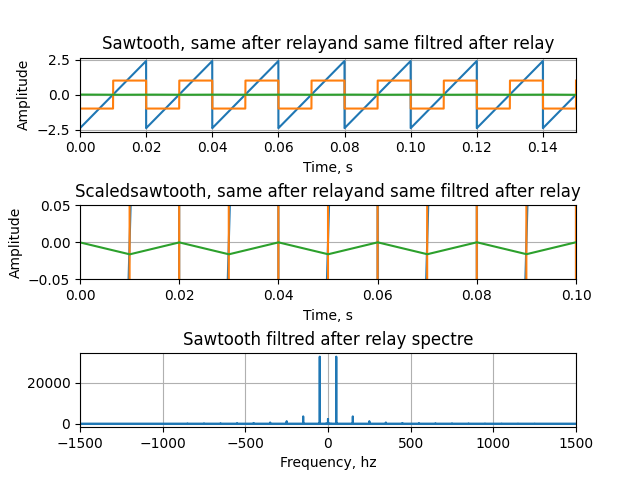
\includegraphics[width=0.95\linewidth]{body/images/sawtooth-after-filtred-relay-and-its-spectre.png}
	\caption{График пилы, отклика нелинейности и отклик линейного звена на преобразованный
	нелинейностью сигнал. Спектр отклика линейного звена}
	\label{fig:24}
\end{figure}

На рис. \ref{fig:24} представлена пила, она же после прохождения
нелинейности \textquotedblleftИдеальное реле\textquotedblright\ и пила,
пропущенная последовательно через нелинейность
\textquotedblleftИдеальное реле\textquotedblright\ и 
линейное фильтрующее звено, а также спектр преобразованного сигнала.
После прохождения нелинейности \textquotedblleftИдеальное реле\textquotedblright, а
затем фильтрующего звена, преобразований сигнал становится значительно подавлен,
но не становится монотонной прямой - это видно на детальном рассмотрении сигнала.
Результирующий сигнал напоминает своей формой асимтотически построенную синусоиду,
сдвинутую по фазе на половину периода исходной пилы. Касательно амплитуды,
полученный сигнал значительно потерял в амлитуде. На спектре же его главной
гармоникой по-прежнему остаётся гармоника частоты первоначальной синусоиды,
но мощность этой гармоники значительно уменьшилась. Также и самих гармоник
после фильтрации относительно преобразованной нелинейностью
\textquotedblleftИдеальное реле\textquotedblright\ пилы становится
меньше. Это обусловлено большей схожестью полученного сигнала с каноническим
видом синусоиды, которая смещена на значение равное своей амплитуде.
Заметна и появившаяся невероятно низкочастотная гармоника

\subsubsection{Получение откликов линейного звена на преобразованный
нелинейностью \textquotedblleftМёртвая зона\textquotedblright\ сигнал.
Получение спектров откликов}

\begin{figure}[H]
	\centering
	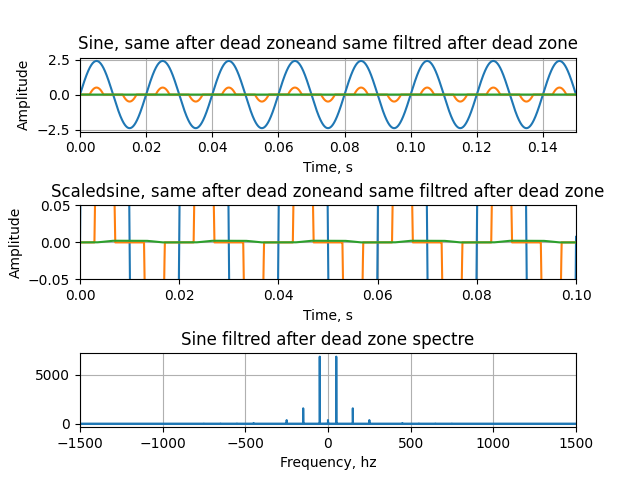
\includegraphics[width=0.95\linewidth]{body/images/sine-after-filtred-dead-zone-and-its-spectre.png}
	\caption{График синусоиды, отклика нелинейности и отклика линейного звена на преобразованный
	нелинейностью сигнал. Спектр отклика линейного звена}
	\label{fig:25}
\end{figure}

На рис. \ref{fig:25} представлена синусоида, она же после прохождения
нелинейности \textquotedblleftМёртвая зона\textquotedblright\ и синусоида,
пропущенная последовательно через нелинейность \textquotedblleftМёртвая зона\textquotedblright\
и линейное фильтрующее звено, а также спектр преобразованного сигнала.
После прохождения нелинейности \textquotedblleftМёртвая зона\textquotedblright, а
затем фильтрующего звена, преобразований сигнал становится значительно подавлен,
но не становится монотонной прямой - это видно на детальном рассмотрении сигнала.
Результирующий сигнал напоминает своей формой асимтотически построенную синусоиду,
сдвинутую по фазе на половину периода исходной синусоиды. Касательно амплитуды,
полученный сигнал значительно потерял в амлитуде. На спектре же его главной
гармоникой по-прежнему остаётся гармоника частоты первоначальной синусоиды,
но мощность этой гармоники значительно уменьшилась. Также и самих гармоник
после фильтрации относительно преобразованной нелинейностью
\textquotedblleftМёртвая зона\textquotedblright\ синусоиды становится
меньше. Это обусловлено большей схожестью полученного сигнала с каноническим
видом синусоиды, которая смещена на значение равное своей амплитуде.
Заметна и появившаяся невероятно низкочастотная гармоника

\begin{figure}[H]
	\centering
	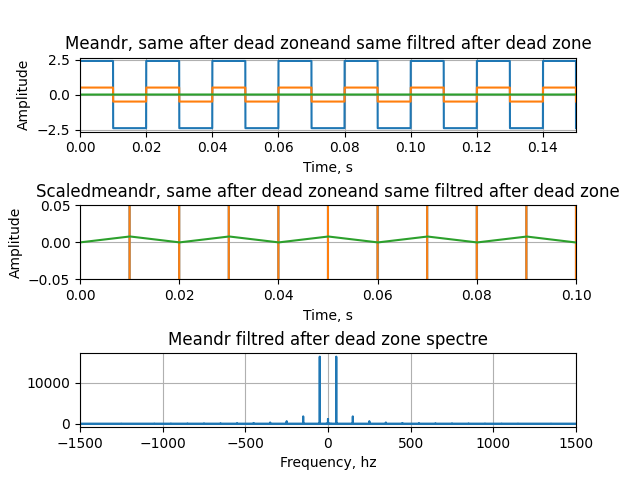
\includegraphics[width=0.95\linewidth]{body/images/meandr-after-filtred-dead-zone-and-its-spectre.png}
	\caption{График меандра, отклика нелинейности и отклика линейного звена на преобразованный
	нелинейностью сигнал. Спектр отклика линейного звена}
	\label{fig:26}
\end{figure}

На рис. \ref{fig:26} представлен меандр, он же после прохождения
нелинейности \textquotedblleftМёртвая зона\textquotedblright\ и меандр,
пропущенный последовательно через нелинейность
\textquotedblleftМёртвая зона\textquotedblright\ и 
линейное фильтрующее звено, а также спектр преобразованного сигнала.
После прохождения нелинейности \textquotedblleftМёртвая зона\textquotedblright\
преобразований сигнал остаётся меандром, который теряет в амплитуде из-за 
свойств нелинейности \textquotedblleftМёртвая зона\textquotedblright.
Полученный после фильтрации сигнал напоминает своей формой асимтотически
построенную синусоиду, сдвинутую по фазе на половину периода исходного меандра.
На спектре же его главной гармоникой по-прежнему остаётся гармоника частоты
первоначального меандра, но мощность этой гармоники значительно уменьшилась.
Также и самих гармоник после фильтрации относительно преобразованного нелинейностью
\textquotedblleftМёртвая зона\textquotedblright\ меадра становится
меньше. Это обусловлено большей схожестью полученного сигнала с каноническим
видом синусоиды, которая смещена на значение равное своей амплитуде.
Заметна и появившаяся невероятно низкочастотная гармоника

\begin{figure}[H]
	\centering
	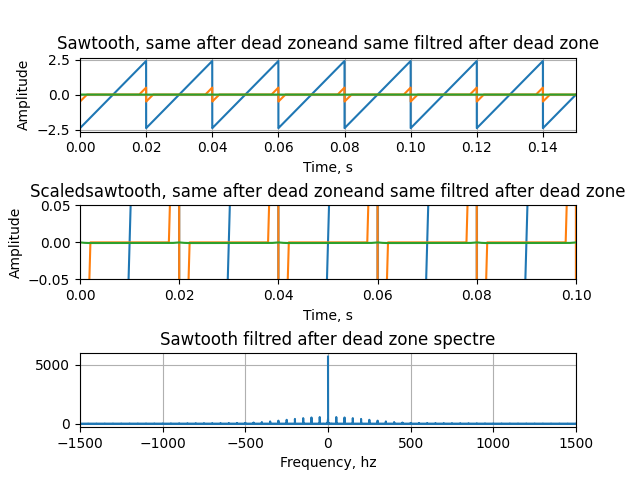
\includegraphics[width=0.95\linewidth]{body/images/sawtooth-after-filtred-dead-zone-and-its-spectre.png}
	\caption{График пилы, отклика нелинейности и отклика линейного звена на преобразованный
	нелинейностью сигнал. Спектр отклика линейного звена}
	\label{fig:27}
\end{figure}

На рис. \ref{fig:27} представлена пила, она же после прохождения
нелинейности \textquotedblleftМёртвая зона\textquotedblright\ и пила,
пропущенная последовательно через нелинейность
\textquotedblleftМёртвая зона\textquotedblright\ и 
линейное фильтрующее звено, а также спектр преобразованного сигнала.
После прохождения нелинейности \textquotedblleftМёртвая зона\textquotedblright, а
затем фильтрующего звена, преобразований сигнал становится подавляется практически
полностью, но не становится монотонной прямой, но всё же стремится к ней. Касательно
амплитуды, полученный сигнал потерял пректически всё значение ампилитуды. На спектре
же его главной гармоникой становится гармоника, близкая к нулечастотной. Остальные
гармоники сохраняют качественный вид гармоник исходной пилы, но встречаются реже

\subsubsection{Получение откликов линейного звена на преобразованный
нелинейностью \textquotedblleftНасыщение\textquotedblright\ сигнал.
Получение спектров откликов}

\begin{figure}[H]
	\centering
	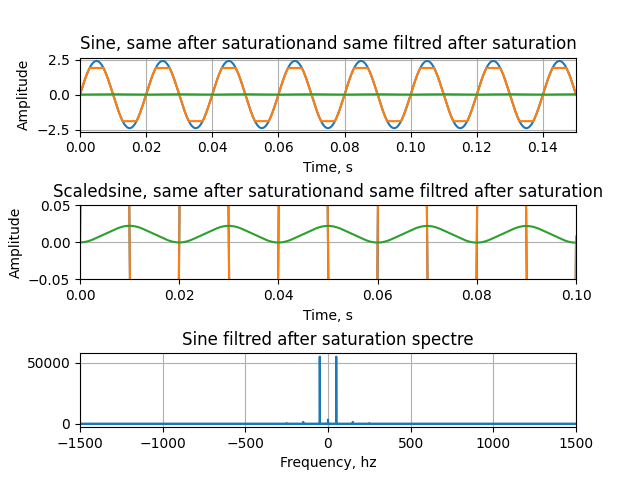
\includegraphics[width=0.95\linewidth]{body/images/sine-after-filtred-saturation-and-its-spectre.png}
	\caption{График синусоиды, отклика нелинейности и отклика линейного звена на преобразованный
	нелинейностью сигнал. Спектр отклика линейного звена}
	\label{fig:28}
\end{figure}

На рис. \ref{fig:28} представлена синусоида, она же после прохождения
нелинейности \textquotedblleftНасыщение\textquotedblright\ и синусоида,
пропущенная последовательно через нелинейность \textquotedblleftНасыщение\textquotedblright\
и линейное фильтрующее звено, а также спектр преобразованного сигнала.
Полученный после фильтрации сигнал остаётся синусоидой с сильно 
уменьшенной амплитудой. Эта синусоида сдвинута по фазе на половину периода исходной
синусоиды. На спектре же её главной гармоникой по-прежнему остаётся гармоника частоты
первоначальной синусоиды, но также появляются и низкочастотные, высокочастотные
маломощные гармоники

\begin{figure}[H]
	\centering
	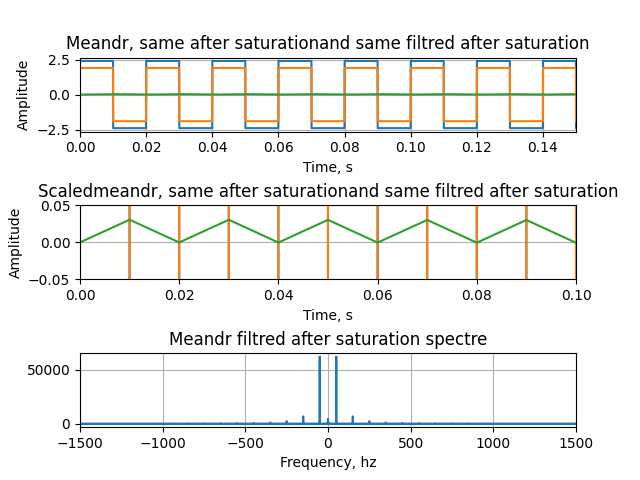
\includegraphics[width=0.95\linewidth]{body/images/meandr-after-filtred-saturation-and-its-spectre.png}
	\caption{График меандра, отклика нелинейности и отклика линейного звена на преобразованный
	нелинейностью сигнал. Спектр отклика линейного звена}
	\label{fig:29}
\end{figure}

На рис. \ref{fig:29} представлен меандр, он же после прохождения
нелинейности \textquotedblleftНасыщение\textquotedblright\ и меандр,
пропущенный последовательно через нелинейность
\textquotedblleftНасыщение\textquotedblright\ и 
линейное фильтрующее звено, а также спектр преобразованного сигнала.
После прохождения нелинейности \textquotedblleftНасыщение\textquotedblright\
преобразований сигнал остаётся меандром, который незначительно теряет в амплитуде
из-за свойств нелинейности \textquotedblleftНасыщение\textquotedblright.
Полученный после фильтрации сигнал напоминает своей формой асимтотически
построенную синусоиду, сдвинутую по фазе на половину периода исходного меандра.
На спектре же его главной гармоникой по-прежнему остаётся гармоника частоты
первоначального меандра, но мощность этой гармоники значительно уменьшилась.
Также и самих гармоник после фильтрации относительно преобразованного нелинейностью
\textquotedblleftНасыщение\textquotedblright\ меадра становится
меньше. Это обусловлено большей схожестью полученного сигнала с каноническим
видом синусоиды, которая смещена на значение равное своей амплитуде.
Заметна и появившаяся невероятно низкочастотная гармоника

\begin{figure}[H]
	\centering
	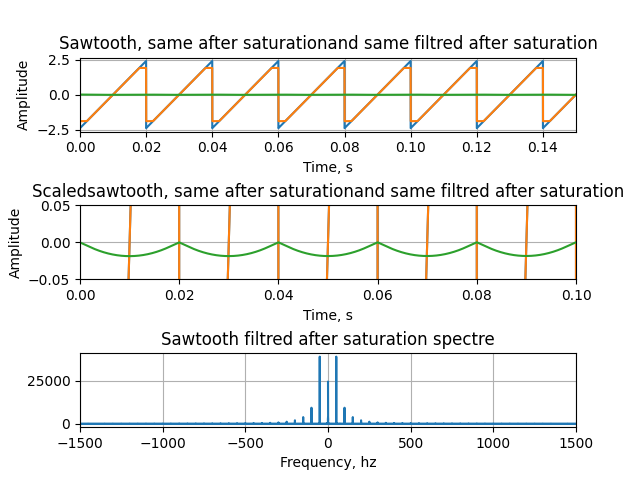
\includegraphics[width=0.95\linewidth]{body/images/sawtooth-after-filtred-saturation-and-its-spectre.png}
	\caption{График пилы, отклика нелинейности и отклика линейного звена на преобразованный
	нелинейностью сигнал. Спектр отклика линейного звена}
	\label{fig:30}
\end{figure}

На рис. \ref{fig:30} представлена пила, она же после прохождения
нелинейности \textquotedblleftНасыщение\textquotedblright\ и пила,
пропущенная последовательно через нелинейность
\textquotedblleftНасыщение\textquotedblright\ и 
линейное фильтрующее звено, а также спектр преобразованного сигнала.
После прохождения нелинейности \textquotedblleftМёртвая зона\textquotedblright, а
затем фильтрующего звена, преобразований сигнал становится похож на конкатинацию
сегментов круга. Спектр полученного сигнала отдалённо напоминает качественный вид
спектра исходной пилы, прошедней через нелинейность
\textquotedblleftНасыщение\textquotedblright: Главная гармоник не является самой
низкочастотной, все гармоники теряют в мощности, а низкочастотные гармоники
подавляются тем сильнее, чем мощнее их изначальная мощность

\subsection{Получение откликов нелинейного звена на преобразованный
линейным звеном сигнал. Получение спектров откликов}

\subsubsection{Получение откликов нелинейности
\textquotedblleftИдеальное реле\textquotedblright\ преобразованный
линейным звеном сигнал. Получение спектров откликов}

\begin{figure}[H]
	\centering
	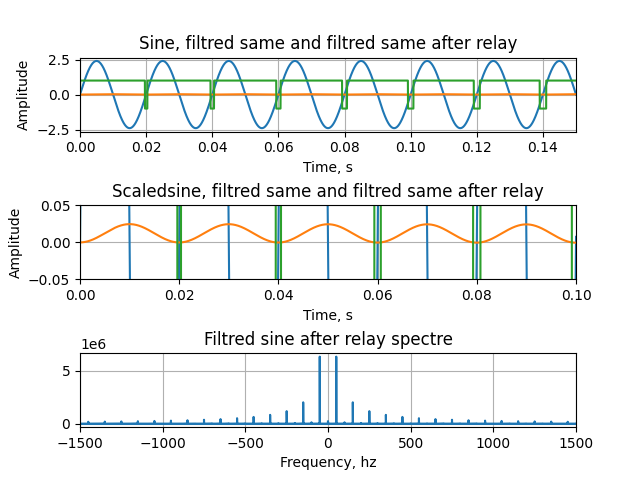
\includegraphics[width=1.05\linewidth]{body/images/filtred-sine-after-relay-and-its-spectre.png}
	\caption{График синусиоды, отклика линейного звена и отклика нелинейности на преобразованный
	линейным звеном сигнал. Спектр отклика нелинейности}
	\label{fig:31}
\end{figure}

На рис. \ref{fig:31} представлена синусоида, она же после прохождения
линейного фильтрующего и синусоида, пропущенная последовательно через линейное
фильтрующее звено и нелинейность \textquotedblleftИдеальное реле\textquotedblright,
а также спектр преобразованного сигнала. После фильтрации синусоида теряет в амплитуде,
а также сдвигается по фазе на половину периода. Также она вздымается ввысь на значение
своей амплитуды. После преобразования нелинейностью
\textquotedblleftИдеальное реле\textquotedblright\ сигнал представляет собой меандр
с уменьшащейся с каждым периодом скважностью или, если говорить по-другому,
увеличивающимся с каждым периодом коэффициентом заполнения. Это видно на графике:
расстояние между преходами меандра увеличиваются с течением времени. 
Амплитуда теряет в соответствии с преобразованием сигнала нелинейностью
\textquotedblleftИдеальное реле\textquotedblright. Спектр
напоминает спектр меандра с гармониками, мощность которых такая же, как мощность
гармоник синусоиды, пропущенной через нелинейность
\textquotedblleftИдеальное реле\textquotedblright. Также на всех частотах: и на
низких, и на высоких, - появляются дополнительные маломощные гармоники

\begin{figure}[H]
	\centering
	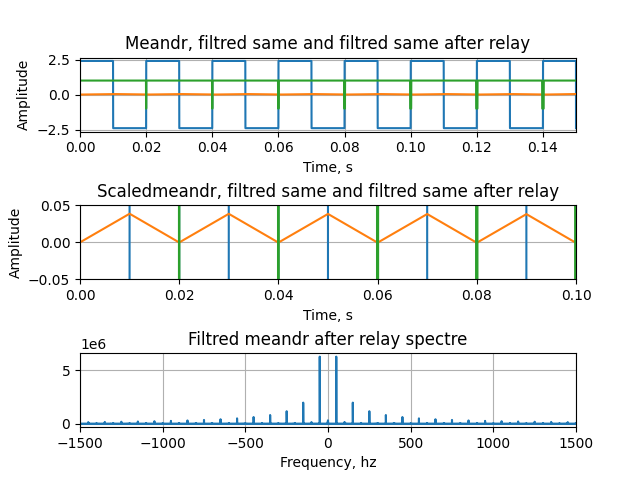
\includegraphics[width=1.05\linewidth]{body/images/filtred-meandr-after-relay-and-its-spectre.png}
	\caption{График меандра, отклика линейного звена и отклика нелинейности на преобразованный
	линейным звеном сигнал. Спектр отклика нелинейности}
	\label{fig:32}
\end{figure}

На рис. \ref{fig:32} представлен меандр, он же после прохождения
линейного фильтрующего и меандр, пропущенный последовательно через линейное
фильтрующее звено и нелинейность \textquotedblleftИдеальное реле\textquotedblright,
а также спектр преобразованного сигнала. После фильтрации меандр теряет в амплитуде,
а также сдвигается по фазе на половину периода. Также он вздымается ввысь на значение
своей амплитуды. Сигнал после фильтрации представляет собой асимтотически построенную
синосоиду. После преобразования нелинейностью \textquotedblleftИдеальное реле\textquotedblright\
сигнал представляет собой меандр с уменьшащейся с каждым периодом скважностью или, если
говорить по-другому, увеличивающимся с каждым периодом коэффициентом заполнения.
Это видно на графике: расстояние между преходами меандра увеличиваются с течением времени. 
Амплитуда теряет в соответствии с преобразованием сигнала нелинейностью
\textquotedblleftИдеальное реле\textquotedblright. Спектр
напоминает спектр меандра с гармониками, мощность которых такая же, как мощность
гармоник синусоиды, пропущенной через нелинейность
\textquotedblleftИдеальное реле\textquotedblright. Также на всех частотах: и на
низких, и на высоких, - появляются дополнительные маломощные гармоники

\begin{figure}[H]
	\centering
	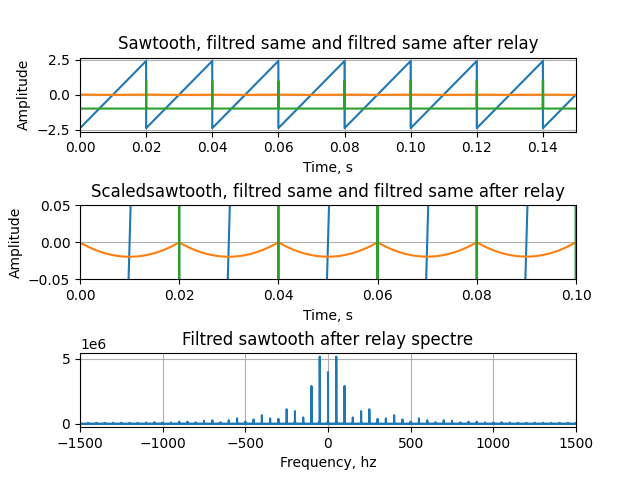
\includegraphics[width=1.05\linewidth]{body/images/filtred-sawtooth-after-relay-and-its-spectre.png}
	\caption{График пилы, отклика линейного звена и отклика нелинейности на преобразованный
	линейным звеном сигнал. Спектр отклика нелинейности}
	\label{fig:33}
\end{figure}

На рис. \ref{fig:33} представлена пила, она же после прохождения
линейного фильтрующего и пила, пропущенная последовательно через линейное
фильтрующее звено и нелинейность \textquotedblleftИдеальное реле\textquotedblright,
а также спектр преобразованного сигнала. После фильтрации пила теряет в амплитуде,
а также сдвигается по фазе на половину периода. Также она опускается на значение
своей амплитуды. Сигнал после фильтрации представляет представляет собой
конкатинацию сегментов круга. После преобразования нелинейностью
\textquotedblleftИдеальное реле\textquotedblright\ сигнал представляет собой меандр
с уменьшащейся с каждым периодом скважностью или, если говорить по-другому, увеличивающимся
с каждым периодом коэффициентом заполнения. Амплитуда теряет в соответствии с
преобразованием сигнала нелинейностью \textquotedblleftИдеальное реле\textquotedblright.
Спектр представляет собой комбинацию \textquotedblleftхолмов\textquotedblright,
образовынный разночастотными гармониками

\subsubsection{Получение откликов нелинейности
\textquotedblleftМёртвая зона\textquotedblright\ преобразованный
линейным звеном сигнал. Получение спектров откликов}

\begin{figure}[H]
	\centering
	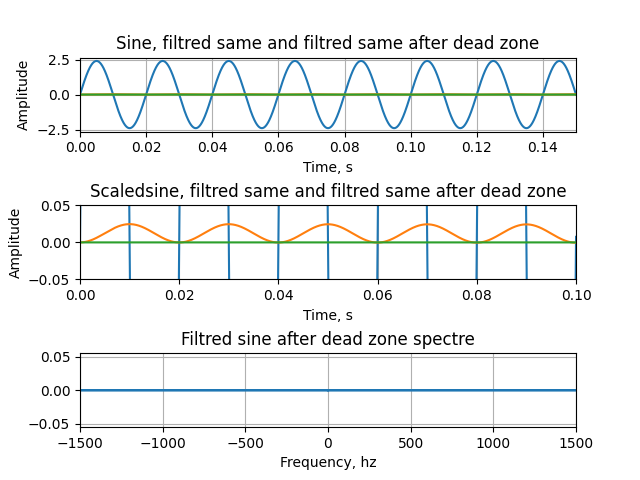
\includegraphics[width=1.05\linewidth]{body/images/filtred-sine-after-dead-zone-and-its-spectre.png}
	\caption{График синусиоды, отклика линейного звена и отклика нелинейности на преобразованный
	линейным звеном сигнал. Спектр отклика нелинейности}
	\label{fig:34}
\end{figure}

На рис. \ref{fig:34} представлена синусоида, она же после прохождения
линейного фильтрующего и синусоида, пропущенная последовательно через линейное
фильтрующее звено и нелинейность \textquotedblleftМёртвая зона\textquotedblright,
а также спектр преобразованного сигнала. После фильтрации синусоида теряет в амплитуде,
а также сдвигается по фазе на половину периода. Также она вздымается ввысь на значение
своей амплитуды. После преобразования нелинейностью
\textquotedblleftМёртвая зона\textquotedblright\ сигнал представляет собой монотонную
прямую. Это связано с тем, что после фильтрации сигнал уже подавлен настолько, что
просто-напросто выходит за пределы мёртвой зоны. Все гармоники в следствие этого 
зануляются. Из-за нулевых гармоник спектр представляет собой гладь без пиков гармоник

\begin{figure}[H]
	\centering
	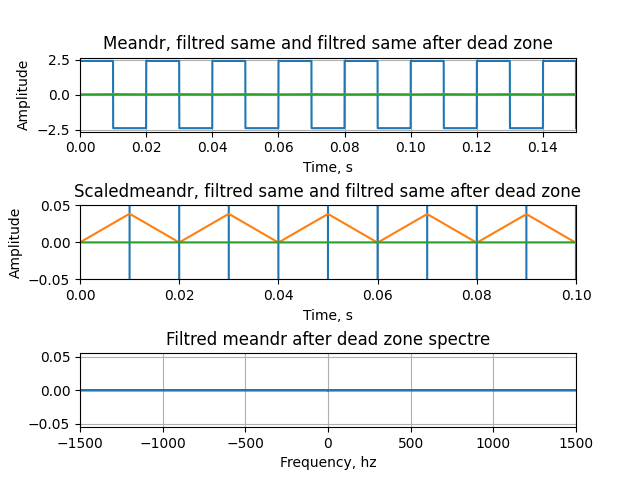
\includegraphics[width=1.05\linewidth]{body/images/filtred-meandr-after-dead-zone-and-its-spectre.png}
	\caption{График меандра, отклика линейного звена и отклика нелинейности на преобразованный
	линейным звеном сигнал. Спектр отклика нелинейности}
	\label{fig:35}
\end{figure}

На рис. \ref{fig:35} представлен меандр, он же после прохождения
линейного фильтрующего и меандр, пропущенный последовательно через линейное
фильтрующее звено и нелинейность \textquotedblleftМёртвая зона\textquotedblright,
а также спектр преобразованного сигнала. После фильтрации меандр теряет в амплитуде,
а также сдвигается по фазе на половину периода. Также он вздымается ввысь на значение
своей амплитуды. Сигнал после фильтрации представляет собой асимтотически построенную
синосоиду. После преобразования нелинейностью
\textquotedblleftМёртвая зона\textquotedblright\ сигнал представляет собой монотонную
прямую. Это связано с тем, что после фильтрации сигнал уже подавлен настолько, что
просто-напросто выходит за пределы мёртвой зоны. Все гармоники в следствие этого 
зануляются. Из-за нулевых гармоник спектр представляет собой гладь без пиков гармоник

\begin{figure}[H]
	\centering
	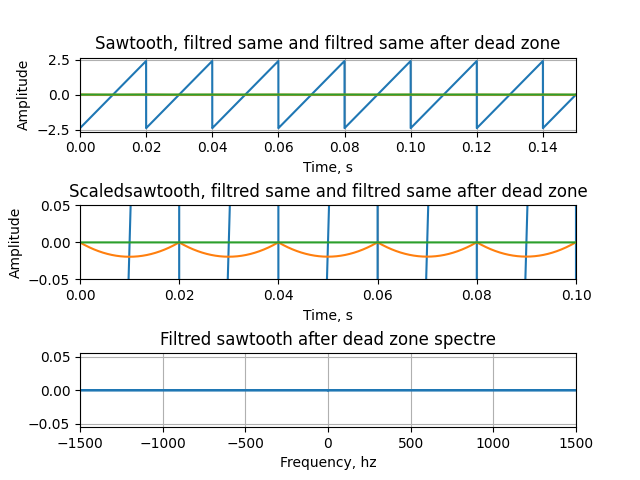
\includegraphics[width=1.05\linewidth]{body/images/filtred-sawtooth-after-dead-zone-and-its-spectre.png}
	\caption{График пилы, отклика линейного звена и отклика нелинейности на преобразованный
	линейным звеном сигнал. Спектр отклика нелинейности}
	\label{fig:36}
\end{figure}

На рис. \ref{fig:36} представлена пила, она же после прохождения
линейного фильтрующего и пила, пропущенная последовательно через линейное
фильтрующее звено и нелинейность \textquotedblleftМёртвая зона\textquotedblright,
а также спектр преобразованного сигнала. После фильтрации пила теряет в амплитуде,
а также сдвигается по фазе на половину периода. Также она опускается на значение
своей амплитуды. Сигнал после фильтрации представляет представляет собой
конкатинацию сегментов круга. После преобразования нелинейностью
\textquotedblleftМёртвая зона\textquotedblright\ сигнал представляет собой монотонную
прямую. Это связано с тем, что после фильтрации сигнал уже подавлен настолько, что
просто-напросто выходит за пределы мёртвой зоны. Все гармоники в следствие этого 
зануляются. Из-за нулевых гармоник спектр представляет собой гладь без пиков гармоник

\subsubsection{Получение откликов нелинейности
\textquotedblleftНасыщение\textquotedblright\ преобразованный
линейным звеном сигнал. Получение спектров откликов}

\begin{figure}[H]
	\centering
	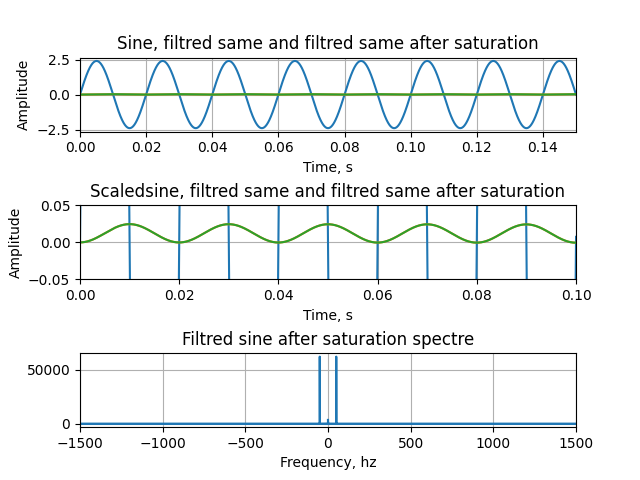
\includegraphics[width=1.05\linewidth]{body/images/filtred-sine-after-saturation-and-its-spectre.png}
	\caption{График синусиоды, отклика линейного звена и отклика нелинейности на преобразованный
	линейным звеном сигнал. Спектр отклика нелинейности}
	\label{fig:37}
\end{figure}

На рис. \ref{fig:37} представлена синусоида, она же после прохождения
линейного фильтрующего и синусоида, пропущенная последовательно через линейное
фильтрующее звено и нелинейность \textquotedblleftНасыщение\textquotedblright,
а также спектр преобразованного сигнала. После фильтрации синусоида теряет в амплитуде,
а также сдвигается по фазе на половину периода. Также она вздымается ввысь на значение
своей амплитуды. Так как амплитуда сигнала после фильтрации невероятно мала, то
нелинейность \textquotedblleftНасыщение\textquotedblright\ не может заметно повлиять
на сигнал, вследствие чего сигнал остаётся без изменений. Это видно и на спектре:
никаких дополнительных гармоник не появляется. Спектр остаётся таким же, как и после
прохождения сигналом линейного фильтрационного звена. Рассматривая спектр, можно
сказать, что на нём видно только уменьшение мощности гармоник. Новых гармоник по
сравнению с сигналом, пропущенным через линейное фильтрующее звено, не наблюдается

\begin{figure}[H]
	\centering
	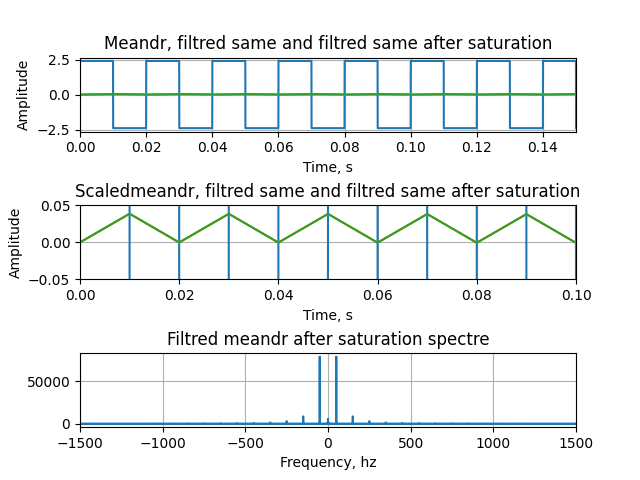
\includegraphics[width=1.05\linewidth]{body/images/filtred-meandr-after-saturation-and-its-spectre.png}
	\caption{График меандра, отклика линейного звена и отклика нелинейности на преобразованный
	линейным звеном сигнал. Спектр отклика нелинейности}
	\label{fig:38}
\end{figure}

На рис. \ref{fig:38} представлен меандр, он же после прохождения
линейного фильтрующего и меандр, пропущенный последовательно через линейное
фильтрующее звено и нелинейность \textquotedblleftНасыщение\textquotedblright,
а также спектр преобразованного сигнала. После фильтрации меандр теряет в амплитуде,
а также сдвигается по фазе на половину периода. Также он вздымается ввысь на значение
своей амплитуды. Сигнал после фильтрации представляет собой асимтотически построенную
синосоиду. Так как амплитуда сигнала после фильтрации невероятно мала, то
нелинейность \textquotedblleftНасыщение\textquotedblright\ не может заметно повлиять
на сигнал, вследствие чего сигнал остаётся без изменений. Это видно и на спектре:
никаких дополнительных гармоник не появляется. Спектр остаётся таким же, как и после
прохождения сигналом линейного фильтрационного звена. Рассматривая спектр, можно
сказать, что на нём видно только уменьшение мощности гармоник. Новых гармоник по
сравнению с сигналом, пропущенным через линейное фильтрующее звено, не наблюдается

\begin{figure}[H]
	\centering
	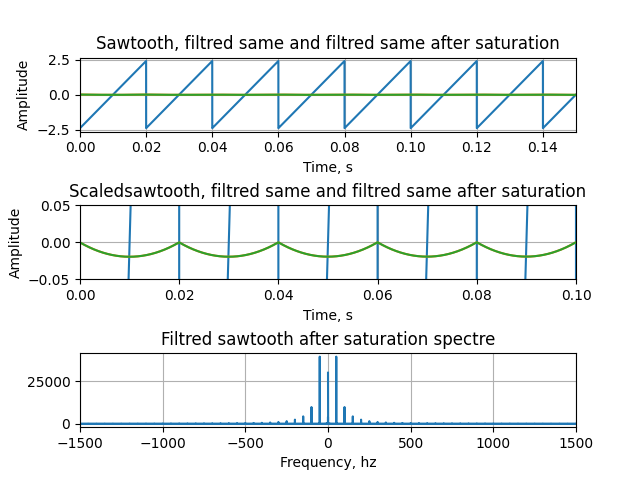
\includegraphics[width=1.05\linewidth]{body/images/filtred-sawtooth-after-saturation-and-its-spectre.png}
	\caption{График пилы, отклика линейного звена и отклика нелинейности на преобразованный
	линейным звеном сигнал. Спектр отклика нелинейности}
	\label{fig:39}
\end{figure}

На рис. \ref{fig:39} представлена пила, она же после прохождения
линейного фильтрующего и пила, пропущенная последовательно через линейное
фильтрующее звено и нелинейность \textquotedblleftНасыщение\textquotedblright,
а также спектр преобразованного сигнала. После фильтрации пила теряет в амплитуде,
а также сдвигается по фазе на половину периода. Также она опускается на значение
своей амплитуды. Сигнал после фильтрации представляет представляет собой
конкатинацию сегментов круга. Так как амплитуда сигнала после фильтрации невероятно мала, то
нелинейность \textquotedblleftНасыщение\textquotedblright\ не может заметно повлиять
на сигнал, вследствие чего сигнал остаётся без изменений. Это видно и на спектре:
никаких дополнительных гармоник не появляется. Спектр остаётся таким же, как и после
прохождения сигналом линейного фильтрационного звена. Рассматривая спектр, можно
сказать, что на нём видно только уменьшение мощности гармоник. Новых гармоник по
сравнению с сигналом, пропущенным через линейное фильтрующее звено, не наблюдается

\section{Выводы}

В ходе выполнения лабораторной работы были изучены основные виды
нелинейностей: \textquotedblleftИдеальное реле\textquotedblright,
\textquotedblleftМёртвая зона\textquotedblright,
\textquotedblleftНасыщение\textquotedblright. Также было
рассмотрено их влияние на три типа пробных сигналов: синусоида,
меандр, пилообразный сигнал. Были рассмотрены отклики нелинейностей
на каждый из пробный сигналов, а также рассмотрены их спектры.
Из полученных данных установлено, что нелинейность
\textquotedblleftИдеальное реле\textquotedblright\ преобразует сигналы
в меандр с амплитудой, равной 1; нелинейность
\textquotedblleftМёртвая зона\textquotedblright\ не меняет форму
сигнала, но уменьшает его амплитуду; нелинейность
\textquotedblleftНасыщение\textquotedblright\ обрезает сигналы.

Были получены статические характеристики нелинейностей. При формировании
статической характеристики синусоида каждый раз отображала характеристику,
аналогичную теоретической. При формировании статической характеристики
меандр каждый раз отображал наклонную линии, форма которой связана с
мгновенным изменением значений сигнала. При формировании статической
характеристики пила каждый раз отображала комбинацию двух вышеописанных
характеристик. 

Опираясь на результаты комбинации НЭ-ЛЗ можно сказать, что синусоида,
как правило, приобретал высокочастотные гармоники, меандр сохранял
все гармоники, а пила либо приобретала низкочастотные, либо терял
высокочастотные.

Опираясь на результаты комбинации ЛЗ-НЭ можно сказать, что
нелинейность \textquotedblleftИдеальное реле\textquotedblright\ 
нивелировало работу фильтра, каждый раз формируя меандр.
Нелинейность \textquotedblleftИдеальное реле\textquotedblright\  
полностью гасила сигнал. Нелинейность 
\textquotedblleftНасыщение\textquotedblright\ практически никак не
влияла на полученный после фильтрации сигнал

Также в дополнение к самой работе, были изучены возможности языка
программирования Python. Был разработан код для формирования всех сигналов,
который можно увидеть в репозитории \href{https://github.com/MaxAizy/TAC/tree/lab1}{github}